% !TEX root = hazelnut-dynamics.tex

\subsection{Example 1: Evaluating Past Holes and Hole Closures}

Consider the perspective of a teacher in the midst of developing a \Hazel{} notebook
to compute final student grades at the end of a course.
Fig.~\ref{fig:grades-cell-mockup} depicts the cell containing the incomplete program that 
the teacher has written so far (we omit irrelevant parts of the UI). 
%

At the top of this program, the teacher defines a
record type, \lismall{Student}, for recording a student's course data---here,
the student's name, of type
\lismall{string}, and, for simplicity, three grades, each of type \lismall{float}. Next, the teacher constructs a list of student records, binding it to the variable \lismall{students}. For simplicity, we include only three example students.
At the bottom of the program, the teacher maps a function \li{weighted_average} over this student data (\li{map} is the standard map function over lists, not shown), intending to compute a final weighted average for each student.
However, the program is incomplete because the teacher has not yet completed the body of the \lismall{weighted_average} function. This pattern is quite common: programmers often consume a function before implementing it.

Thusfar in the body of \lismall{weighted_average}, the teacher has decomposed the function argument into variables by record destructuring, then multiplied the homework grade, \li{hw}, by \li{30.0} and finally inserted the \li{+} operator. The cursor now sits at an \emph{empty hole}, as indicated by the vertical bar and the green background. Each hole has a unique name (generated automatically in \Hazel), here simply \li{1}. 
%In this case, there is only one hole in the program, but in general, there may be many such holes.

Let us briefly digress: in a conventional ``batch'' programming system, writing \li{30.0*hw +} by itself would simply cause parsing to fail and there would be no static or dynamic feedback.
In response, the programmer might encode a hole by raising an exception. This would cause typechecking to succeed. 
However, 
evaluation would proceed only as far as the first \li{map} iteration, 
which would call into \li{weighted_average} and then fail when attempting to evaluate the hole.%
\footnote{In a lazy language, like Haskell, the result would be much the same because the environment forces the result for printing.}
% While the stack trace would confirm that \li{weighted_average} has been called, this is not entirely satisfying.

\Hazel{} does not take this ``exceptional'' interpretation of holes. Instead, evaluation continues past the hole, treating it as an opaque expression of the appropriate type. The result, shown at the bottom of Fig.~\ref{fig:grades-cell-mockup}, is a list of length $3$, confirming that \li{map} does indeed behave as expected in this regard despite the teacher having provided an incomplete argument. Furthermore, each element of the resulting list has been evaluated as far as possible, i.e. the arithmetic expression \li{30.0*hw} has been evaluated for each corresponding value of \li{hw}, as expected. Evaluation cannot proceed any further because holes appear as addends. We say that each of these addition expressions is an \emph{indeterminate} sub-expression, and the result as a hole is therefore also indeterminate, because it is not yet a value, nor can it take a step due to holes in elimination positions.

At this point, the teacher might take notice of the magnitude of the numbers being computed, e.g. \li{2640.0} and \li{2280.0}, and
realize immediately that a mistake has been made: the teacher wants to compute a 
weighted average between \li{0.0} and \li{100.0}, and so the correct
constant is \li{0.30}, not \li{30.0}. %(There are of course other possible fixes.)

Although these observations might 
save only a small amount of time in this case, 
% relative to the 
% situation where the teacher notices this mistake only once  
% the \li{weighted_average} function has been completed, 
it demonstrates
the broader motivations of live programming: continuous feedback about the dynamic behavior of the 
program can help confirm the mental model 
that the programmer has developed (in this case, regarding the behavior of \li{map}), and also help quickly dispel 
misconceptions about the 
actual behavior of the program (in this case, the magnitude of the arithmetic expressions being computed).

% The result itself is not the only live feedback that \Hazel reports to the programmer.
% Programmers also keep track of the names and types of the variables that are in scope at the cursor. 
Going further, \Hazel helps programmers reason about the dynamic behavior of expressions bound to variables in scope at a hole via the \emph{live context inspector}, normally displayed  as a sidebar but shown disembodied in three states in Fig.~\ref{fig:grades-sidebar}. 
In all three states, the live context inspector displays the names and types of the variables that are in scope. 
New to our approach are the values associated with bindings, which come from the environment associated with the selected hole instance in the result. 
We call a hole instance paired with an  environment a \emph{hole closure}, by analogy to function closures (and also due to the logical connection detailed in Sec.~\ref{sec:calculus}). 
In this case, there are three instances of hole \li{1} in the result, numbered sequentially \li{1:1}, \li{1:2} and \li{1:3}, arising from the three calls to \li{weighted_averages} by \li{map}. 
% An environment is a partial mapping of variables in scope to values. 
The programmer can directly select different closures by clicking on a hole instance in the result (the first instance, \li{1:1}, is selected by default, as indicated by the purple outline in Fig.~\ref{fig:grades-cell-mockup}), or cycle through all of the closures for the hole at the cursor by clicking the arrows at the bottom of the context inspector, e.g. $\blacktriangleright$, or using hotkeys.

\vspace{-4px}
\subsection{Example 2: Recursive Functions}\label{sec:qsort1}\label{sec:paths}
\vspace{-2px}

% !TEX root = hazelnut-dynamics.tex

\begin{figure}[t]
\begin{subfigure}[t]{\textwidth}
\centering
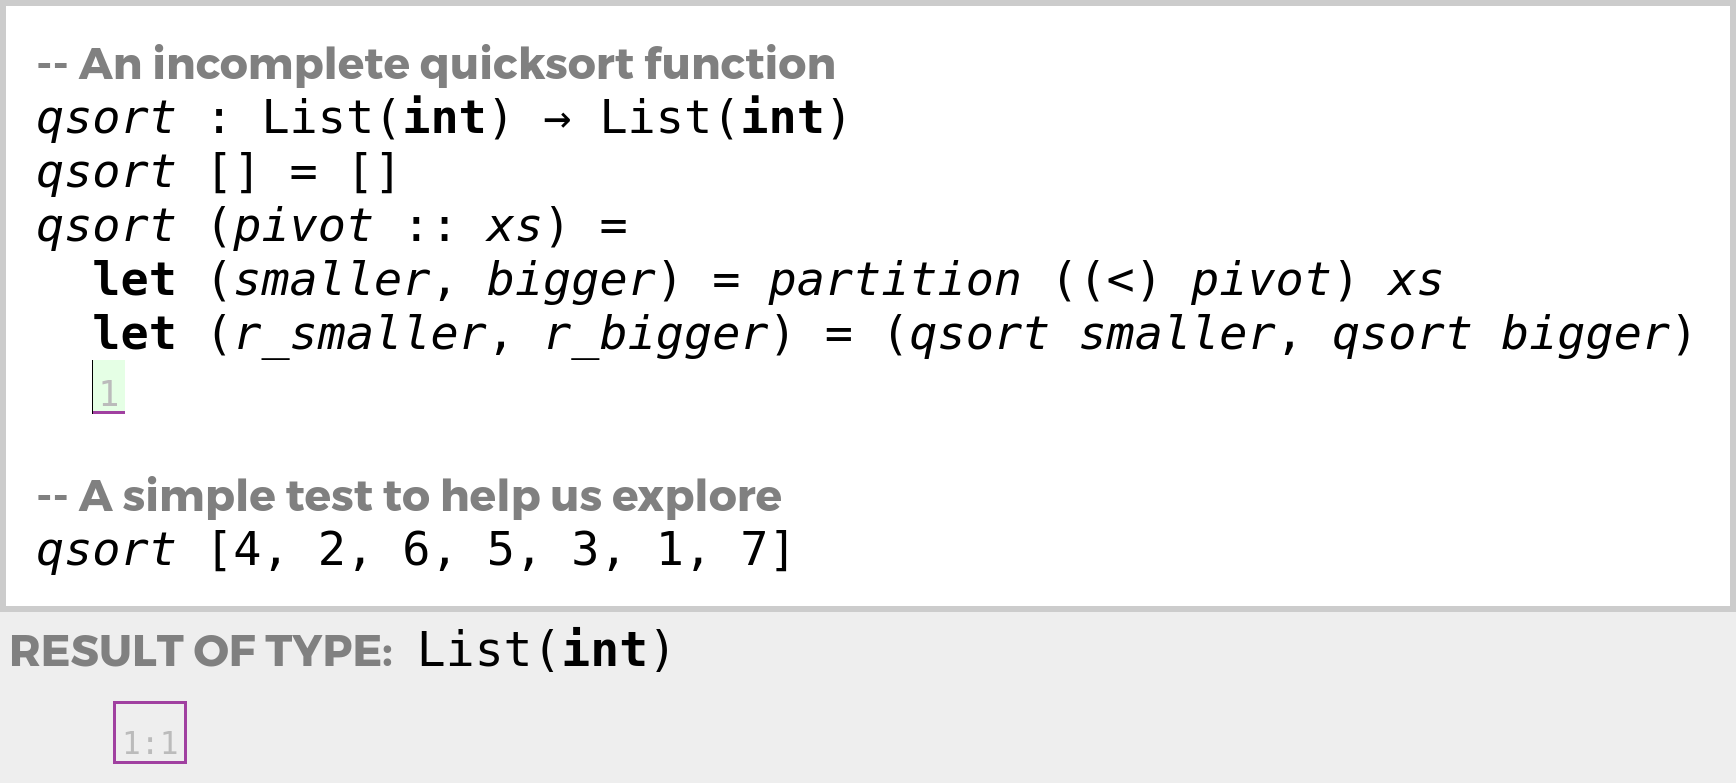
\includegraphics[width=0.57\textwidth,interpolate=false,valign=t]{images/qsort-code.png}
\vspace{-3px}
\caption{The result of evaluating this incomplete quicksort function applied to a test value is a hole closure.}
\label{fig:qsort-example-code}
\end{subfigure}

\vspace{10px}

\begin{subfigure}[t]{\textwidth}
\centering
\includegraphics[width=0.29\textwidth,interpolate=false,valign=c]{images/qsort-new-sidebar-1.png}
~$\xrightarrow[\text{click}]{}$
\includegraphics[width=0.29\textwidth,interpolate=false,valign=c]{images/qsort-new-sidebar-2.png}
~$\xrightarrow[\text{click}]{}$
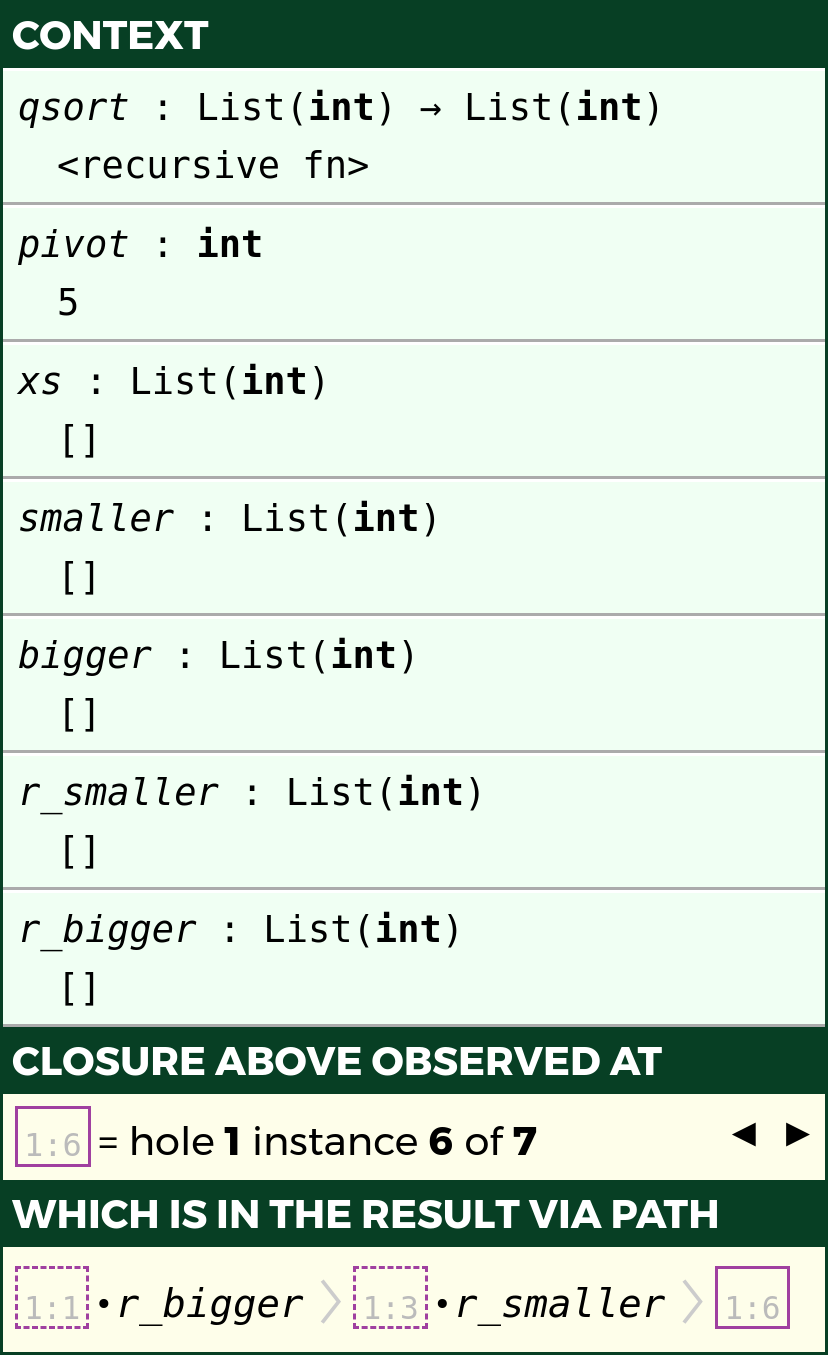
\includegraphics[width=0.29\textwidth,interpolate=false,valign=c]{images/qsort-new-sidebar-3.png}
\caption{The programmer can explore the recursive structure of the computation by clicking on hole instances.}
\label{fig:qsort-sidebars}
\end{subfigure}

\vspace{3px}

\caption{Example 2: Incomplete Quicksort}
\label{fig:qsort-cell-mockup}
% \end{subfigure}
\end{figure}

% \begin{subfigure}[t]{\textwidth}
% \centering
% 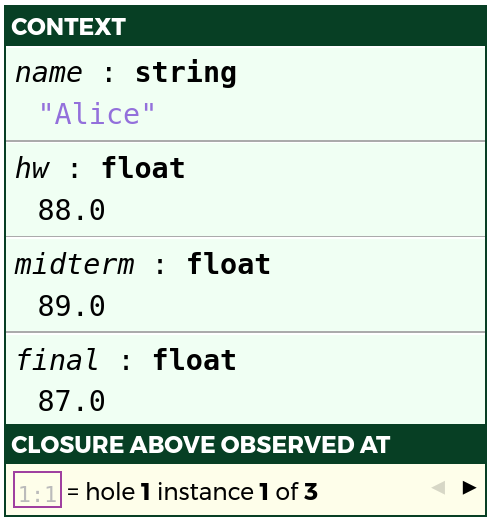
\includegraphics[width=0.3\textwidth,interpolate=false]{images/grades-sidebar-1.png}
% ~${}^\blacktriangleright$
% 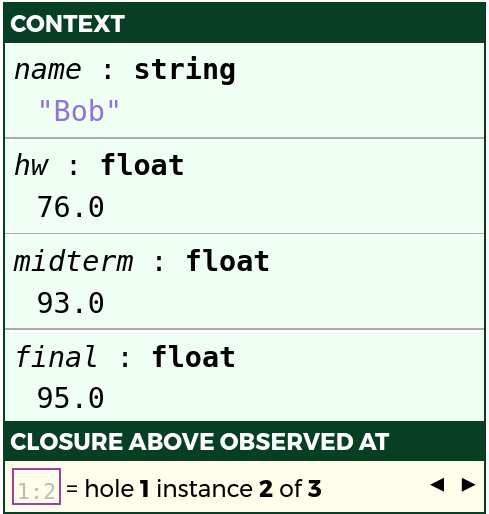
\includegraphics[width=0.3\textwidth,interpolate=false]{images/grades-sidebar-2.png}
% ~${}^\blacktriangleright$
% 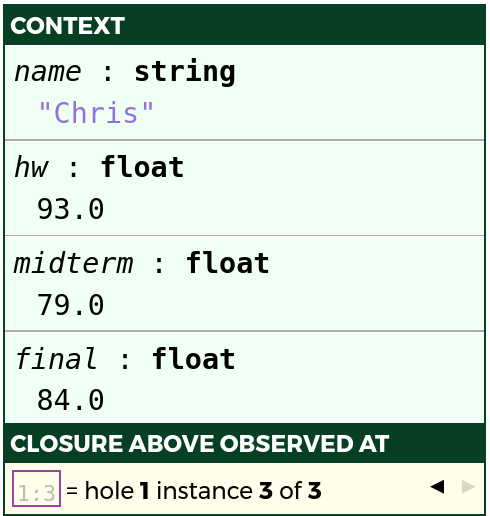
\includegraphics[width=0.3\textwidth,interpolate=false]{images/grades-sidebar-3.png}
% \caption{Typing context view with live hole closure information}
% \label{sec:grades-sidebar}
% \end{subfigure}
% %% TODO once the code above is removed, scale up the screenshots
% 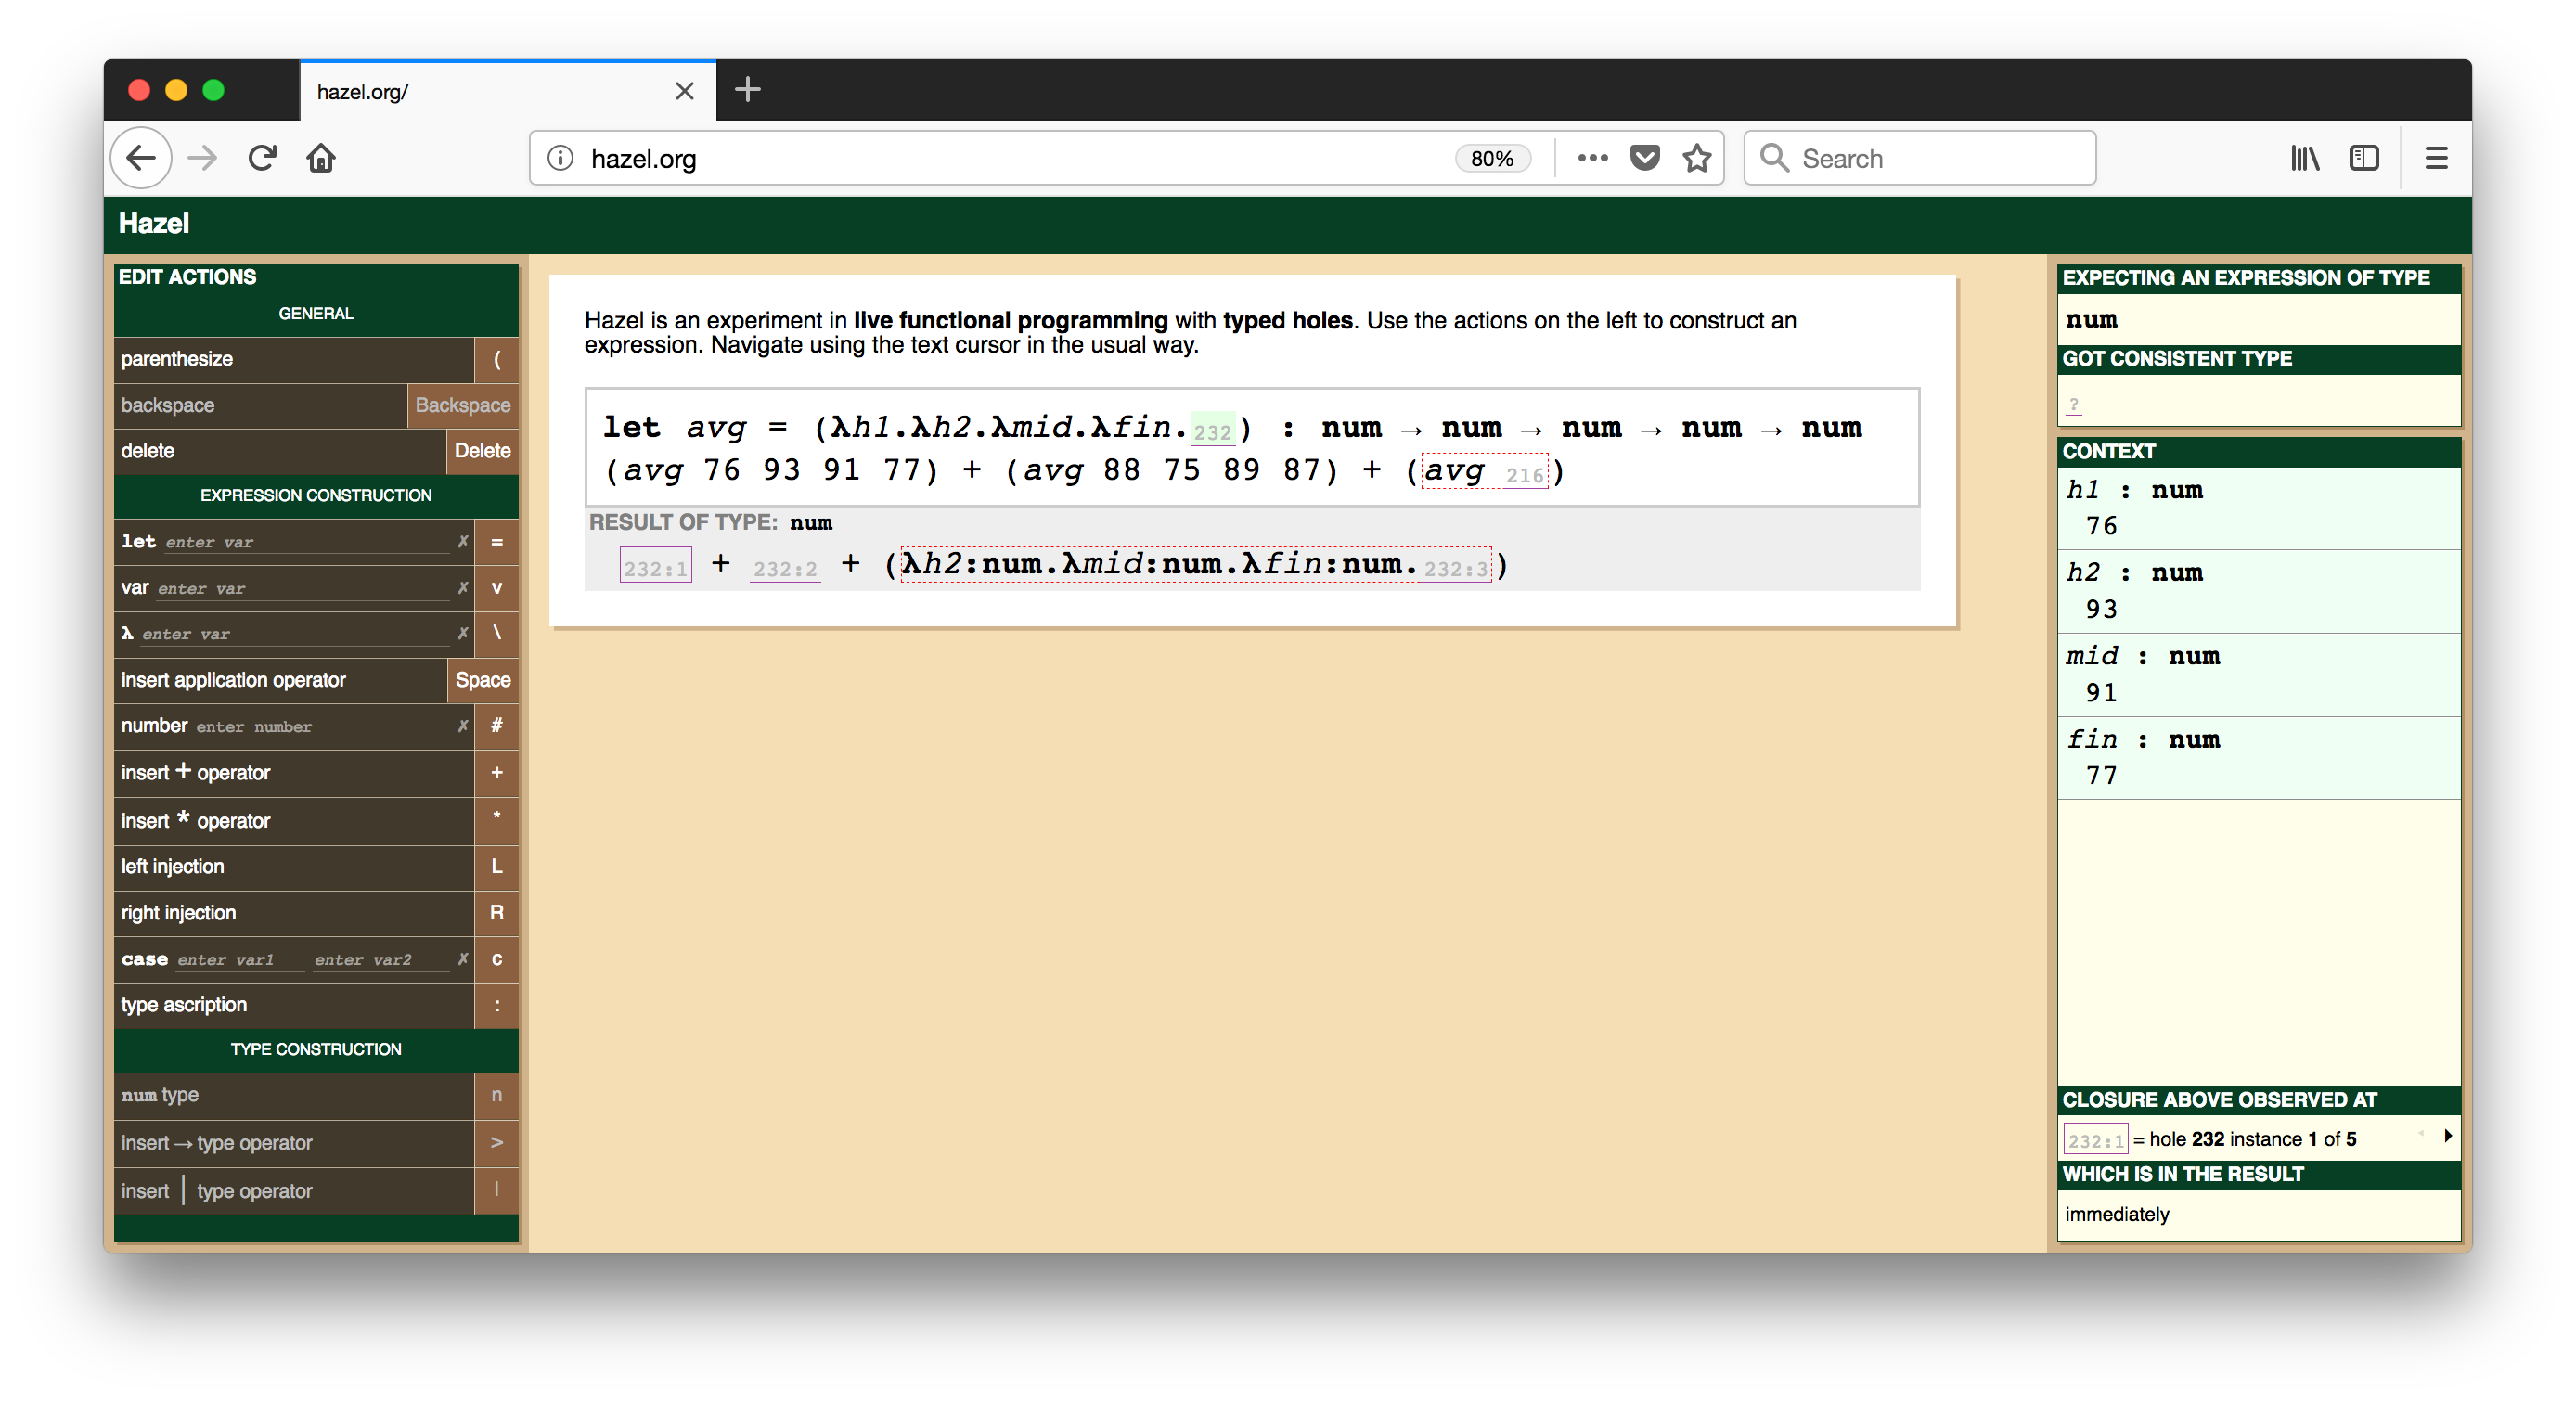
\includegraphics[scale=0.20]{images/hazel-placeholder-0.png}

% \rkc{Draw arrows and captions on the top figure to show how to get
% to the bottom figure.
% ser navigates to hole a, types + to create a plus, types * to create a
% multiplication, types \#10 to create 10, types vh1 to create variable use.}

% 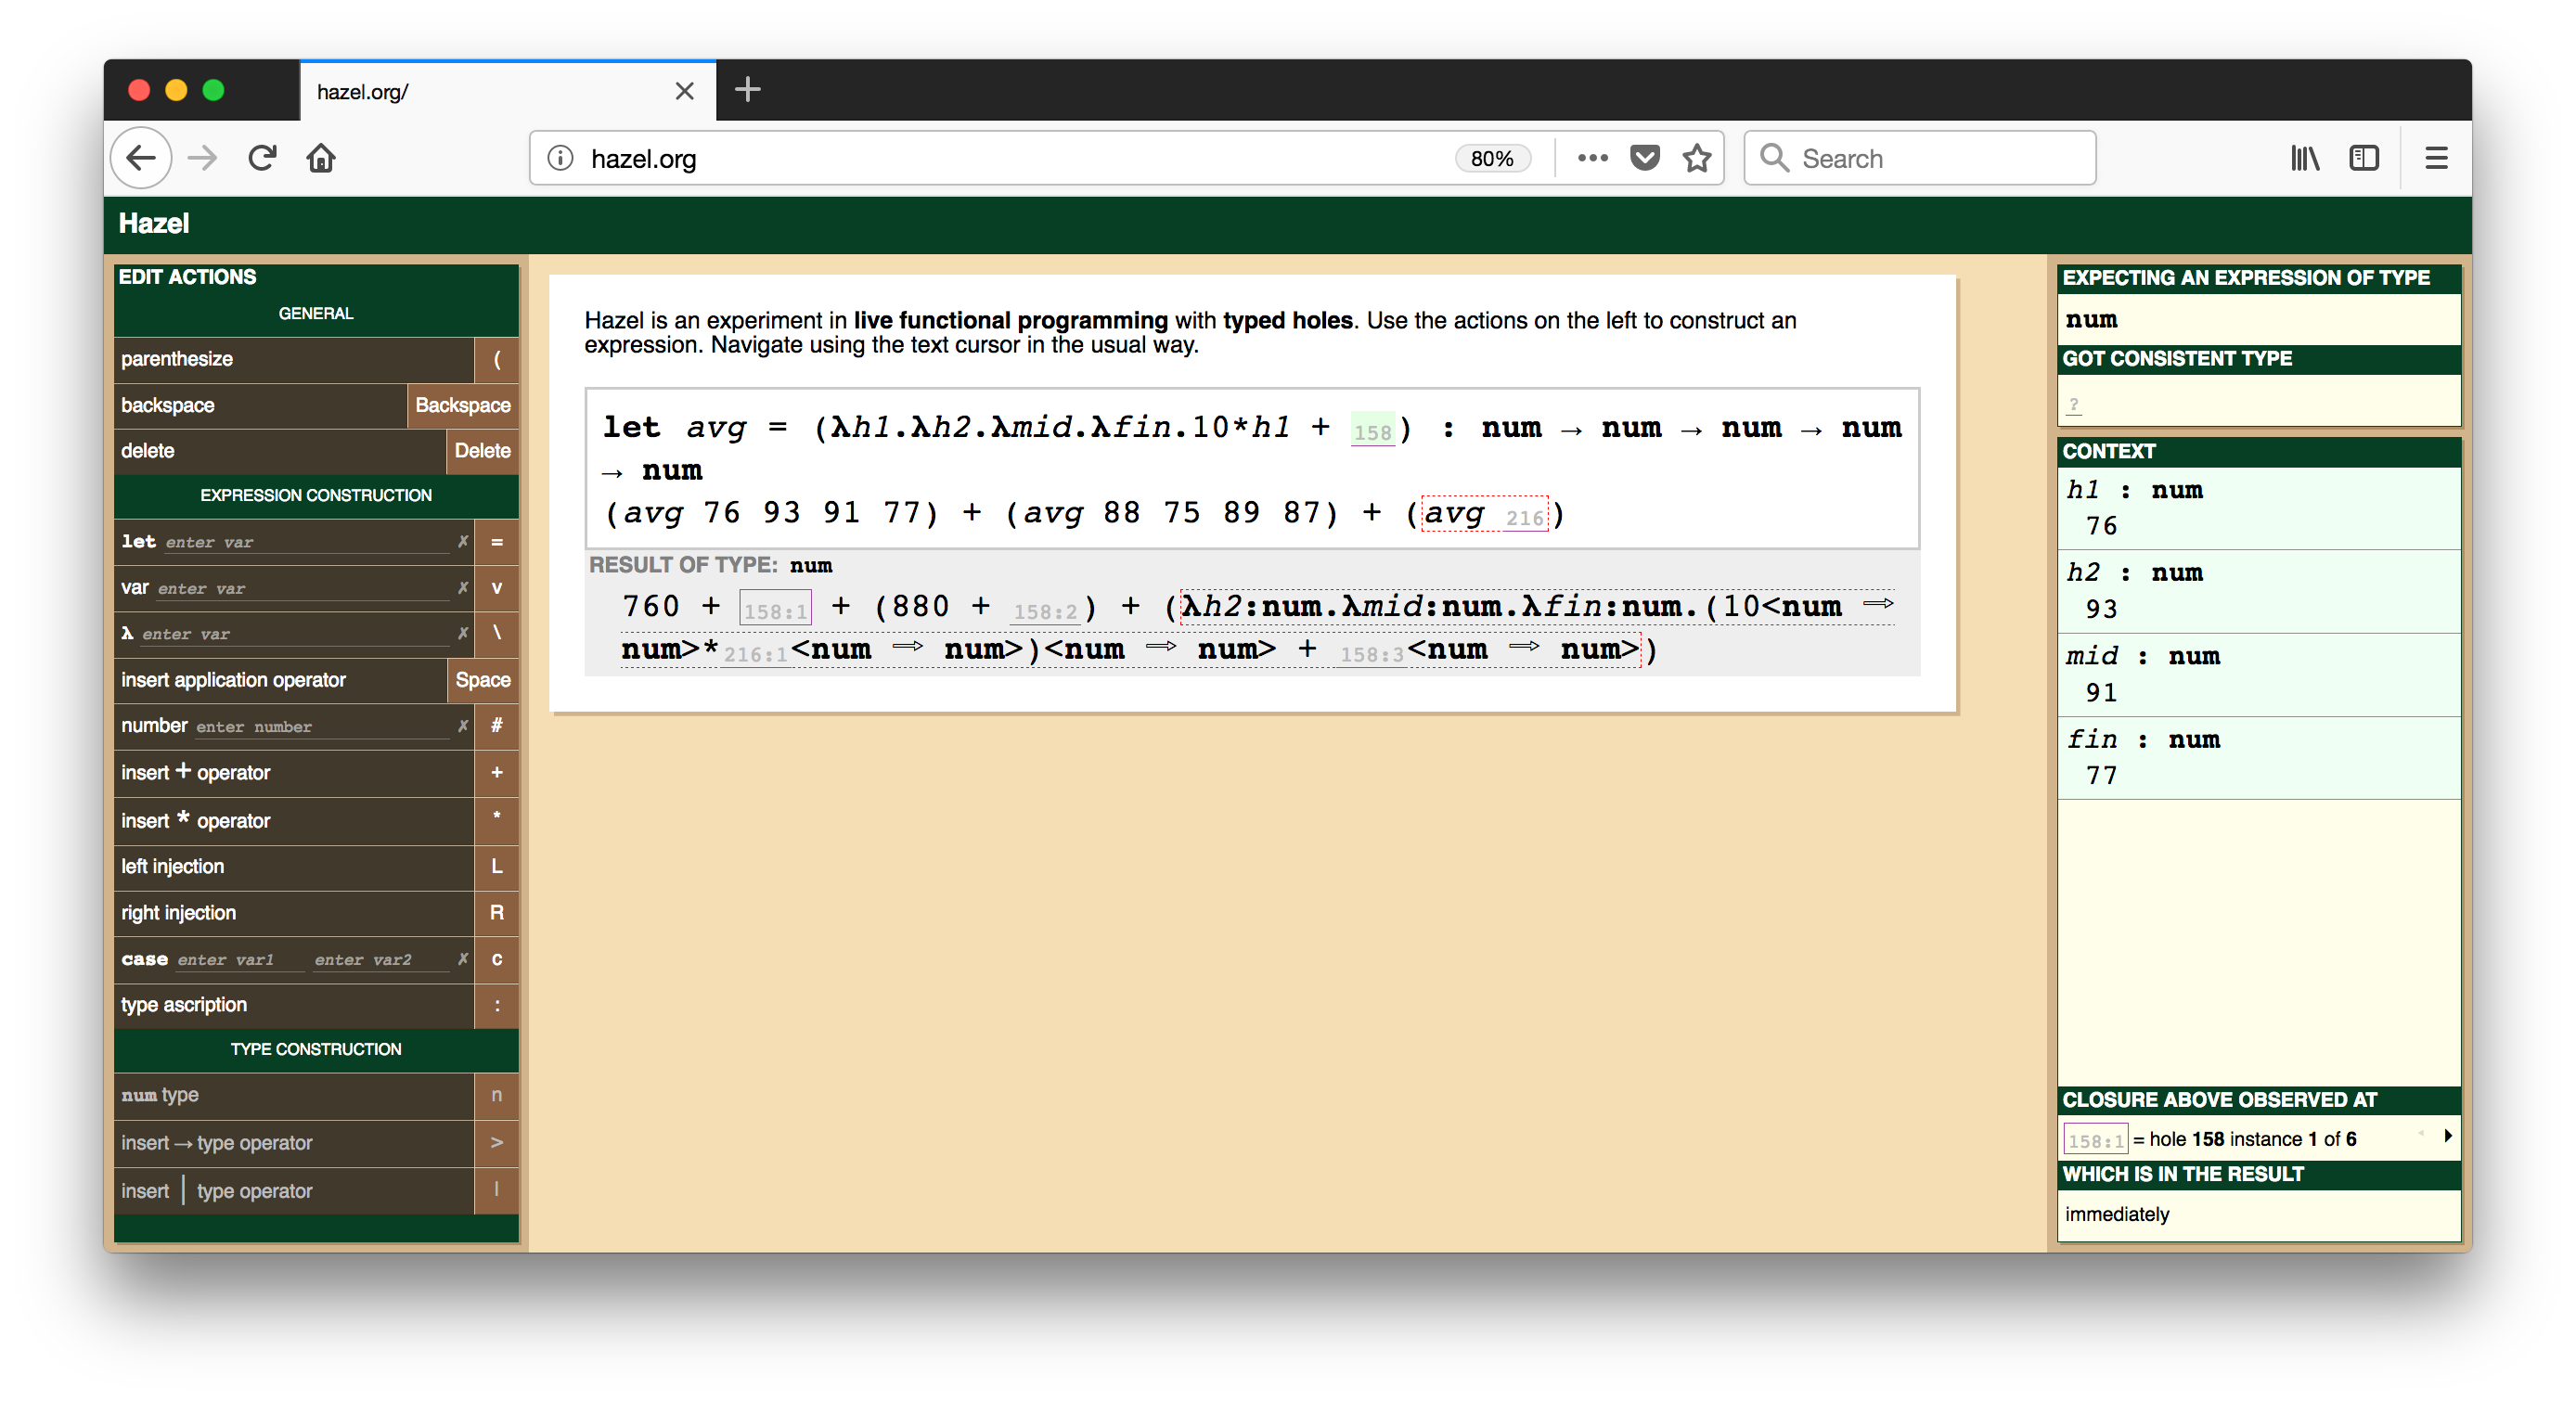
\includegraphics[scale=0.20]{images/hazel-placeholder-1a.png}


Let us now consider a second more sophisticated example: an incomplete implementation of the recursive quicksort function, shown in Fig.~\ref{fig:qsort-example-code}. So far, the programmer (perhaps a student, or a lecturer using \Hazel as a presentational aid) has filled in the base case, and in the recursive case, partitioned the remainder of the list relative to the head, and made the two recursive calls. A hole appears in return position as the programmer contemplates how to fill the hole with an appropriate expression of list type, as indicated by the \emph{type inspector} in Fig.~\ref{fig:qsort-type-inspector}.

At the bottom of the cell in Fig.~\ref{fig:qsort-example-code}, the programmer has applied \li{qsort} to an example list. However, 
the indeterminate result of this function application is simply an instance of hole \li{1}, which serves only to confirm that evaluation went through the recursive case of \li{qsort}. 
More interesting is the live context inspector, shown in three states in Fig.~\ref{fig:qsort-sidebars}, which provides feedback about the values of the variables in scope at hole \li{1} from the the various instances of hole \li{1} that appear in the result, either immediately or within an outer closure. For example, in its initial state (Fig.~\ref{fig:qsort-sidebars}, left) it shows the closure at the instance of hole \li{1} that appears immediately in the result due to the outermost application of \li{qsort}. From this, the programmer can confirm (or the lecturer can visually point out) that 
the lists \li{smaller} and \li{bigger} computed by the call to \li{partition} are appropriately named, and observe that they are not yet themselves sorted.

The results from the subsequent recursive calls, \li{r_smaller} and \li{r_bigger}, are again hole instances, \li{1:2} and \li{1:3}. 
The programmer can click on either of these hole instances to reveal the associated closures from the corresponding recursive calls. 
For example, clicking on \li{1:3} reveals the hole closure from the \li{r_bigger} recursive call as shown in Fig.~\ref{fig:qsort-sidebars} (middle). 
From there, the programmer can click another hole closure, e.g. \li{1:6} to reveal the hole closure from the subsequent \li{r_smaller} recursive call as shown in Fig.~\ref{fig:qsort-sidebars} (right). 
Notice in each case that the path from the result to the selected hole closure is reported as shown at the bottom of the context inspector in Fig.~\ref{fig:qsort-sidebars}. 
In exploring these paths rooted at the result, the programmer can develop concrete intuitions about the recursive structure of the computation (e.g. by following through to the base case as shown in Fig.~\ref{fig:qsort-sidebars}) even before the program is complete. 
% (We leave to future work the pedagogical question of whether such early feedback might help students understand recursion.)

\begin{comment}
Now the teacher returns to \lismall{weighted_average} to work on the missing
expression, with the goal of computing a weighted sum of each of a student's
grades.
%
The teacher performs several \Hazel{} edit actions (each of which is a single
keystroke, a shortcut to selecting one of the edit tools from the left panel,
followed by a tool-specific argument terminated with the Enter key):
%
navigating the cursor to hole \lismall{a} and typing \lismall{+}, which creates a
sum expression \lismall{??_b + ??_c} with the cursor placed, by default, under
left operand (the hole labeled \lismall{b});
%
typing \lismall{*} to create a multiplication expression \lismall{??_d * ??_e + ??_c},
with the cursor place under hole \lismall{d};
%
typing \lismall{\#10} to enter a numeric scaling factor, which then moves
the cursor to the second operand, hole \lismall{e}; and
%
typing \lismall{vg.hw1} to use the \lismall{hw1} field of the function argument
as the right operand of the multiplication.
%
The resulting partial expression, \lismall{(10.0 *. g.hw1) +. ??_b}---shown
in the screenshot in the bottom half of \autoref{fig:grades-example}---marks the
first of five weighted summands in the eventual finished \lismall{weighted_average}
calculation.
\end{comment}

\begin{comment}
Each \Hazel{} edit action transforms an incomplete but well-formed and
well-typed program into another such program, and, thus, \Hazel{} immediately
runs the program after each edit.
%
After the above edit sequence, \Hazel{} display the updated list of
indeterminate expressions \lismall{[760.0 + ??_b.1, 880.0 + ??_b.2, ...]}.
%
Right away, the teacher recognizes that the values are too large; they should be
at most \lismall{100.0}.
%
The teacher realizes that representing percentage points as \lismall{float}s requires
that the constant on line \rkc{XXX} ought to be \lismall{0.10} instead.
%
Because of this live feedback, the teacher corrects this error right away and
avoids making similar programming errors in the rest of the calculation.
%
The teacher continues to build the rest of the arithmetic expression until it is
complete (there are no longer any expression holes), and the result of
immediately running the finished program shows that each of values in the final
result list is in the range \lismall{0.0} to \lismall{100.0}.
\end{comment}

\begin{comment}
\begin{figure}[t]

\rkc{Move all this code into the mockup screenshots below.}

\lstset{basicstyle=\scriptsize\ttfamily}
\begin{lstlisting}
type grade_cutoffs =
  { a: float, b: float, c: float, d: float, f: float };

let cutoffs =
  { a = ??_a, b = ??_b, c = ??_c, d = ??_d, f = ??_f };

let letter_grade(n: weighted_average) =
  if n >= cutoffs.a then "A" else
  if n >= cutoffs.b then "B" else
  if n >= cutoffs.c then "C" else
  if n >= cutoffs.d then "D" else
  if n >= cutoffs.f then "F" else "Incomplete";

let sorted_weighted_averages = List.sort weighted_averages;

let letter_grades = List.map letter_grade sorted_weighted_averages;

let compute_distribution(list: list(float)) =
  let n = List.length letter_grades in
  List.map
    (\x -> (x, showPercentage (List.length (List.filter ((==) x) list)) /. n))
    ["A","B","C","D","F","Incomplete"];

let distribution = compute_distribution(letter_grades);
\end{lstlisting}
%% restore settings from main.tex
\lstset{basicstyle=\footnotesize\ttfamily}

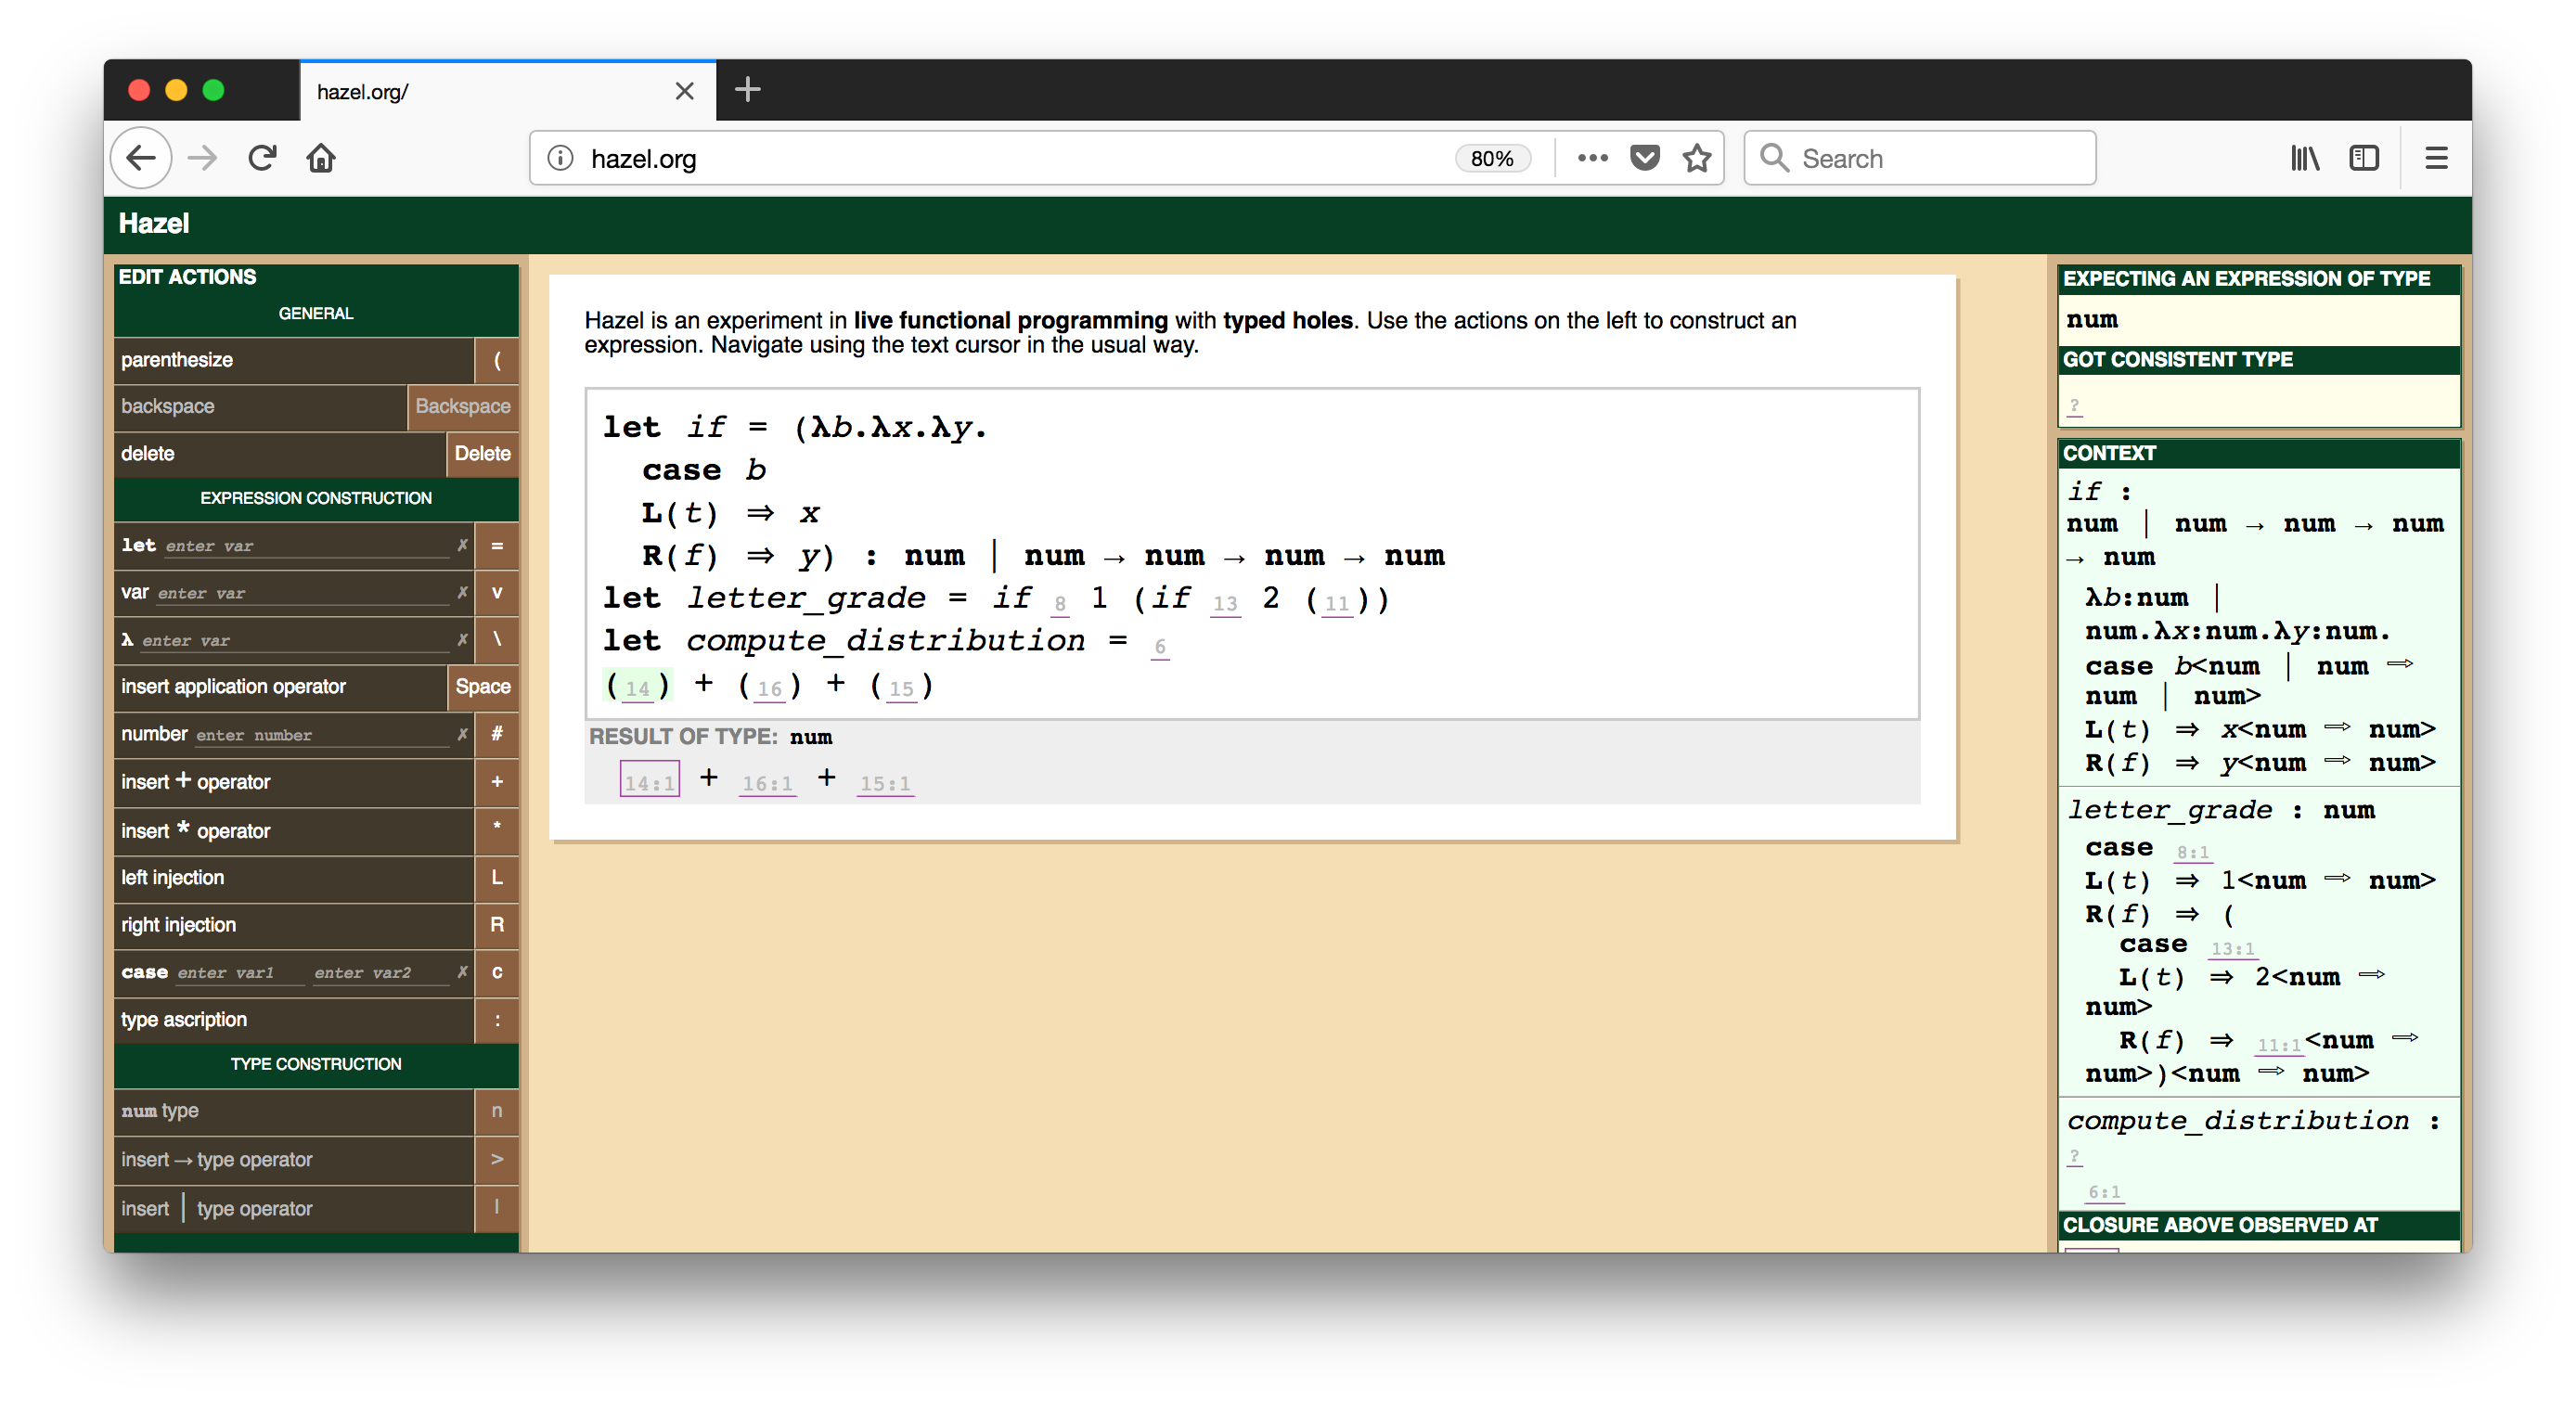
\includegraphics[scale=0.27]{images/hazel-placeholder-1b.png}

\caption{Hazel mockup for Example 1b.}
\label{fig:grades-example-b}
\end{figure}


\overviewExample{1b}{Assigning Letter Grades}
%
The teacher's next task is to map the weighted averages to the letter grades A
through F (we consider only ``whole'' letter grades, for simplicity).
%
The \lismall{grade_cutoffs} record type, shown at the top of
\autoref{fig:grades-example-b}, describes the minimum cutoff for each of
these six possible grades.
%
Initially, each value in the \lismall{cutoffs} record is a hole.

%
%% initially all holes, because it will be different year-to-year based on the %
%data, differences in course difficulty, and to satisfy fairness criteria.
%
Before starting to fill in the cutoff values, the teacher jumps ahead to write a
function \lismall{letter_grade} that will make the connection between \lismall{cutoffs}
and \lismall{weighted_averages}.
%
Because she intends to look at the data to help select the cutoff values, the
teacher sorts the \lismall{weighted_averages} (on line \rkc{XXX}) and then maps
them to \lismall{letter_grades} (on line \rkc{XXX}).

When \Hazel{} runs this program, the guard of the outermost conditional
(\lismall{n >= cutoffs.a} on line \rkc{XXX}), is indeterminate because \lismall{cutoffs.a}
is.
%
Therefore, each of the indeterminate expressions in \lismall{letter_grades} is the
entire expression body, albeit with different bindings for \lismall{n}.
%
Displaying such ``large'' indeterminate expressions can quickly consume all
available screen space, overwhelming the user with too much information.
%
\autoref{fig:XXX} shows how \Hazel{} renders large indeterminate
expressions (\ie{}~anything other than ``small'' indeterminate value (a constant
or hole) or list of small values) simply as \lismall{..} to save space.
%
Hovering over this abbreviation (\rkc{???}) displays the full
indeterminate expression---as well as the evaluation environment that surrounds
it---as a tooltip.
%
\autoref{sec:discussion} discusses this and other user interface concerns when
trying to display useful live feedback without overwhelming the user.
%
These usability factors are beyond the scope of our work, which is to define
semantic foundations on which such user interfaces can be built.

To start deciding \lismall{cutoffs}, the teacher clicks the \lismall{weighted_averages}
expression, and views the results panel to see the data sorted in descending
order.
%
The result shows a natural gap between \lismall{92.2} and \lismall{89.5}.
%
So, she chooses to use \lismall{92.0} as the cutoff for A, replacing hole \lismall{XXX} on
line \rkc{XXX} with that numeric value.
%
Resuming the computation from before, \Hazel{} resolves the conditional
expressions for the first \rkc{XXX} indeterminate expressions, because each of
those \lismall{n} values was greater than \lismall{cutoffs.a}.
%
The remaining \rkc{XXX} expressions also proceeded to evaluate the first guard,
and are now indeterminate at the guard for the second conditional.

Before assigning subsequent cutoff values, the teacher would like to get a sense
of whether this first choice is a good one.
%
She jumps ahead to to write a function (\lismall{compute_distribution} on lines
rkc{XXX}-\rkc{XXX}) that computes the distribution of letter grades based
on \verb+cutoffs+..
%
Running \lismall{compute_distribution} shows that the percentage of As is
\rkc{XXX\%}, which is smaller than what the teacher would like;
the remaining percentages are all indeterminate.
%
Returning to the value of \lismall{sorted_data}, she sees a cluster around \lismall{89.0}
and then another gap between \lismall{88.2} and {85.5}.
%
So, the teacher adjusts \lismall{cutoffs.a} to be \lismall{88.0}.
%
Because this edit is not just filling a hole expression, \Hazel{} discards the
previous execution state and reevaluates the entire program.
%
Existing techniques for incremental computation~\cite{XXX,XXX}, however, could
be applied to seek opportunities for reuse even when non-hole expressions are
modified.
%
Because the focus of work is on the novel implications of running programs with
holes, our calculus and implementation supports caching ``edit-and-resume'' only
for the novel situation in which evaluation proceeds around holes.
%
After re-evaluation, the percentage of As becomes \rkc{XXX\%}, which better
matches the teacher's intention.

In this fashion, the teacher continues down the list of sorted averages,
determining appropriate values for each cutoff.
%
Whenever the teacher is only filling in the ``next'' cutoff, the computation
from before can simply be resumed.
%
Overall, throughout the workflow described in these two examples, the programmer
can continue to evaluate the program, and receive meaningful feedback, while
going back and forth between different pieces under development.
\end{comment}
